\documentclass[11pt]{article}
\usepackage[toc,page]{appendix}
\usepackage{amsmath, amssymb}
\usepackage[utf8]{inputenc}
\usepackage[T1]{fontenc}
\usepackage[style=apa,backend=biber]{biblatex}
%\usepackage{biblatex}
\addbibresource{references.bib}
\usepackage{graphicx}
\usepackage{tikz}
\usetikzlibrary{automata,positioning,shapes.geometric, arrows.meta, fit, backgrounds, calc, chains}
\graphicspath{./images/Easy_Pictures/SMR_MULT_Repackaging}%\usepackage{kpfonts}
\usepackage{float}
\usepackage[margin=1in]{geometry}
\usepackage{cancel}
\usepackage{epsfig}
\usepackage{tikz-3dplot}
\usepackage{darkmode}
\usepackage{dirtytalk}
\usepackage{longtable,booktabs,array}
\usepackage{calc} % for calculating minipage widths
\usepackage[utf8]{inputenc}
\usepackage[T1]{fontenc}
\usepackage{xcolor}
\usepackage{listings}


\usepackage{etoolbox}
\usepackage{hyperref}
\hypersetup{
    colorlinks=true,
    linkcolor=blue,
    filecolor=magenta,      
    urlcolor=cyan,
    pdftitle={Hermeneutic Calculator},
    citecolor=blue,
    }


\urlstyle{same}

\lstdefinestyle{htmlStyle}{
    language=HTML,
    basicstyle=\ttfamily\small,
    keywordstyle=\color{blue}\bfseries,
    commentstyle=\color{gray}\itshape,
    stringstyle=\color{red},
    breaklines=true,
    frame=single,
    numbers=left,
    numberstyle=\tiny\color{gray},
    columns=fullflexible,
}
\lstdefinelanguage{HTML}{
  keywords={<!DOCTYPE, html, head, title, body, h1, h2, h3, p, div, span, a, img, ul, li, table, tr, td, th, style, link, script},
  sensitive=true,
  comment=[l]{//},
  morecomment=[s]{/*}{*/},
  morestring=[b]',
  morestring=[b]"
}
\lstset{style=htmlstyle, language=html}
% Updated to explicitly pass the language option
%\lstinputlisting[style=htmlstyle, language=html]{./html/example.html}
%\usepackage{tocloft}

% Optional: define some custom colors
\definecolor{sliceRed}{RGB}{225,224,91} % matching "varyellow" from your code
\definecolor{linkYellow}{RGB}{255,215,0}  % a golden yellow
\tdplotsetmaincoords{70}{110}

\title{Addition Strategies: Rearranging to Make Bases (RMB)}
\author{Compiled by: Theodore M. Savich}


\begin{document}
\maketitle
\subsection*{Transcript}
Video from \textcite{Carpenter1999}. Strategy descriptions and examples adapted from \textcite{HackenbergCourseNotes}. 
\begin{itemize}
\item \textbf{Teacher:} Lucy is eight fish. She buys five more fish. How many fish will Lucy have then?
\item \textbf{Sarah:}  13. 
\item \textbf{Teacher:} How'd you get 13? 
\item \textbf{Sarah:} Well, because eight plus two is ten, but then two plus three is five. And she wants to buy five more fish. So you take care of two, and you need to add three more. And so I add three more, and you get 13.
\end{itemize}

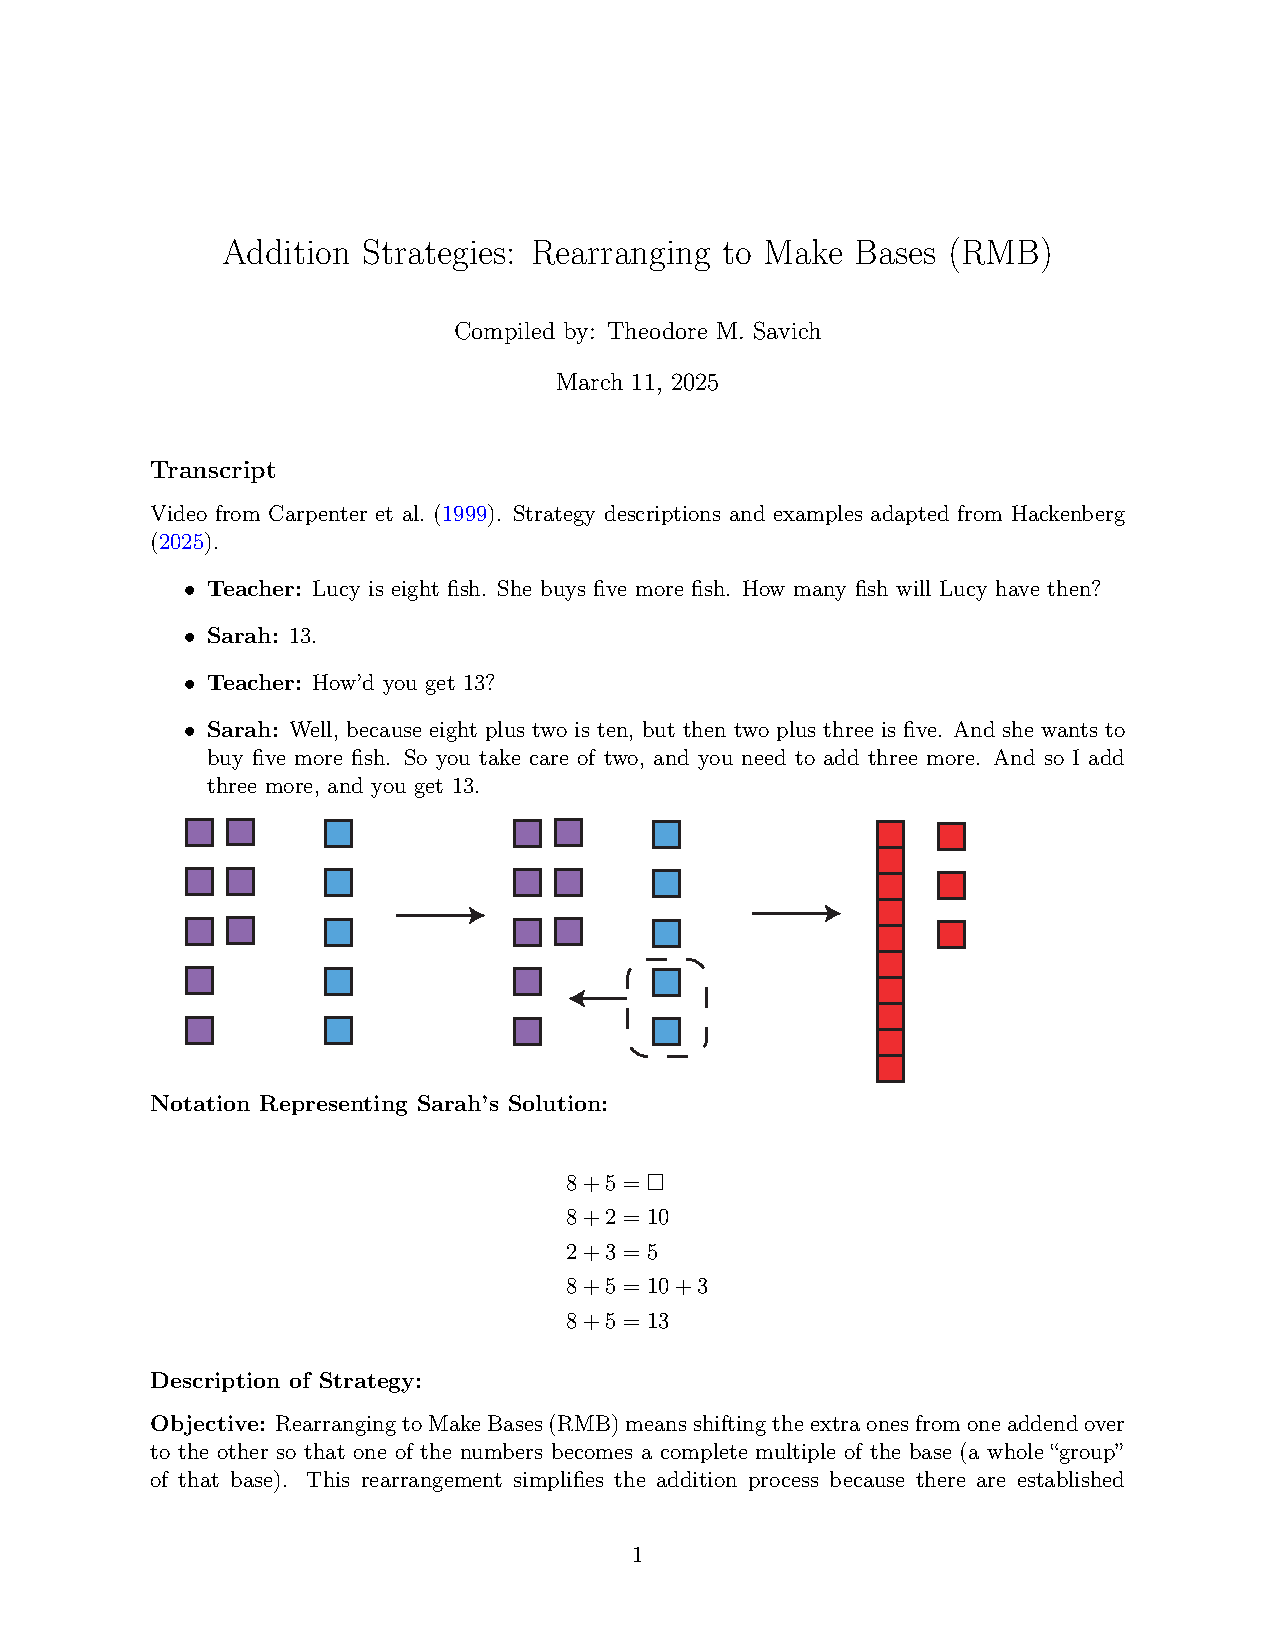
\includegraphics[width=.8\textwidth]{images/Easy_Pictures/SAR_ADD_RMB/PDF/SAR_ADD_RMB.pdf}

\noindent \textbf{Notation Representing Sarah's Solution:}

\begin{align*}
8 + 5 &= \Box \\
8+2 &= 10\\
2+3 &= 5\\
8+5&= 10 + 3\\
8+5 &= 13
\end{align*}

\subsubsection*{Description of Strategy:}

 \textbf{Objective:} Rearranging to Make Bases (RMB) means shifting the extra ones from one addend over to the other so that one of the numbers becomes a complete multiple of the base (a whole ``group'' of that base). This rearrangement simplifies the addition process because there are established patterns for adding an exact multiple of the base. In other words, when you add a full group of base units to a number, the ones digit stays the same while only the digit representing the base (like the tens place) increases.
   

\subsection*{Rearranging to Make Bases (RMB)}

\subsubsection*{Description of Strategy}
\begin{itemize}
    \item \textbf{Objective:} Make one of the addends a whole number of bases by moving ones from the other addend.
    \item \textbf{Example:} \(8 + 5\)
    \begin{itemize}
        \item Move 2 ones from 5 to 8 to make 10.
        \item Remaining ones in the second addend: \(5 - 2 = 3\).
        \item Add the adjusted numbers: \(10 + 3 = 13\).
    \end{itemize}
\end{itemize}

\subsubsection*{Automaton Type}
\textbf{Pushdown Automaton (PDA)}: Needed to handle digits and to remember the number of ones moved via the stack.

\subsubsection*{Rearranging to Make Bases (RMB) Automaton in Python}

The description in `SAR_ADD_RMB.pdf` details how a student (Sarah) solves 8+5 by recognizing that 8 needs 2 to make 10, decomposing 5 into 2+3, and then combining 10+3.

To model this strategy as an \textbf{elaboration of counting}, the following Python implementation uses a Register Machine model. Crucially, it determines the gap (K) and the remainder (R) using iterative counting, reflecting how a student might derive these values without relying on abstract subtraction.

\subsubsection*{Automaton Diagram for RMB}

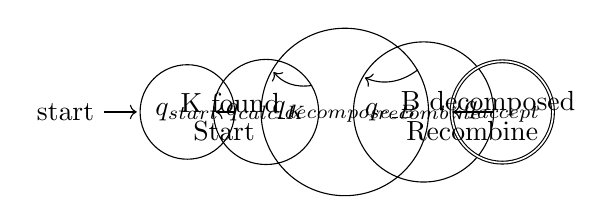
\begin{tikzpicture}[
    shorten >=1pt,
    on grid,
    auto,
    every state/.style={minimum size=1.2cm}
]
    % Define nodes
    \node[state, initial] (start) {$q_{start}$};
    \node[state, right=of start] (calc_k) {$q_{calc\_K}$};
    \node[state, right=of calc_k] (decomp_b) {$q_{decompose\_B}$};
    \node[state, right=of decomp_b] (recombine) {$q_{recombine}$};
    \node[state, accepting, right=of recombine] (accept) {$q_{accept}$};
    
    % Transitions
    \path[->]
        (start) edge node {Start} (calc_k)
        (calc_k) edge[bend left] node {K found} (decomp_b)
        (decomp_b) edge[bend left] node {B decomposed} (recombine)
        (recombine) edge node {Recombine} (accept);
\end{tikzpicture}

\subsubsection*{Python Implementation and Test}
\begin{lstlisting}[language=Python]
import pandas as pd

class RMBAutomatonIterative:
    """
    A Register Machine model simulating the 'Rearranging to Make Bases' (RMB) strategy,
    based on algorithmic elaboration from counting primitives.
    """
    def __init__(self, A, B, Base=10):
        # Heuristic: Apply the strategy to the larger number.
        self.A = max(A, B)
        self.B = min(A, B)
        self.A_initial = self.A
        self.B_initial = self.B
        self.Base = Base

        # Registers for internal computation
        self.K = 0
        self.A_temp = 0 # Used for counting up A
        self.B_temp = 0 # Used for counting down B
        self.Result = 0

        # State
        self.state = 'q_start'
        self.history = []

    def _record_history(self, action, interpretation):
        self.history.append({
            'State': self.state,
            'Action': action,
            'Interpretation': interpretation,
            'A_reg': self.A,
            'B_reg': self.B,
            'K_reg': self.K,
            'A_temp': self.A_temp,
            'B_temp': self.B_temp,
        })

    def transition(self, next_state):
        self.state = next_state

    def run(self):
        # Transition from start directly to calculation
        if self.state == 'q_start':
            self.transition('q_calc_K')

        while self.state not in ['q_accept', 'q_error']:
            if self.state == 'q_calc_K':
                self.execute_calc_K()
            elif self.state == 'q_decompose_B':
                self.execute_decompose_B()
            elif self.state == 'q_recombine':
                self.execute_recombine()
            else:
                self.transition('q_error')
                break

        return self.Result

    def execute_calc_K(self):
        """q_calc_K: Calculate K needed to reach the base by counting up from A."""

        # Determine the target base
        if self.A % self.Base == 0 and self.A != 0:
             target_base = self.A
        else:
             target_base = ((self.A // self.Base) + 1) * self.Base

        if self.A_temp == 0:
            # Initialize
            self.A_temp = self.A
            self.K = 0
            self._record_history("Initialize K calc", f"Start counting up from A ({self.A}) to Target Base ({target_base}).")

        if self.A_temp < target_base:
            # Iterative counting up (Primitive operation)
            self.A_temp += 1
            self.K += 1
            self._record_history("A_temp += 1, K += 1", f"Count up: {self.A_temp}. Distance (K): {self.K}.")
        elif self.A_temp == target_base:
            self._record_history("Reached Target Base", f"K needed is {self.K}.")
            self.transition('q_decompose_B')

    def execute_decompose_B(self):
        """q_decompose_B: Decompose B by counting down K from B."""
        K_needed = self.K

        # Initialize B_temp if K>0 and this is the first entry into the state (A_temp > A)
        if self.K > 0 and self.B_temp == 0 and self.A_temp > self.A:
             self.B_temp = self.B
             self._record_history("Initialize B decomp", f"Start counting down K ({self.K}) from B ({self.B}).")

        if self.K > 0 and self.B_temp > 0:
            # Iterative counting down (Primitive operation)
            self.B_temp -= 1
            self.K -= 1
            self._record_history("B_temp -= 1, K -= 1", f"Transferred 1. B remainder: {self.B_temp}. K remaining: {self.K}.")
        elif self.K == 0:
            # Success: K has been transferred
            self.A = self.A_temp # A is now the target base
            self.B = self.B_temp # B is the remainder
            self._record_history("Decomp Complete", f"Transferred {K_needed}. New state: A={self.A}, B={self.B}.")
            self.transition('q_recombine')
        elif self.K > 0 and self.B_temp == 0:
            # Failure: B was insufficient
            self._record_history("Strategy Failed", f"B ({self.B_initial}) is too small to provide K ({K_needed}).")
            self.transition('q_error')

    def execute_recombine(self):
        """q_recombine: Combine the new A (base) and the remainder B."""
        # This step exploits the base structure (cognitively easy)
        self.Result = self.A + self.B
        self._record_history("Result = A + B", f"Combine rearranged numbers: {self.A} + {self.B} = {self.Result}.")
        self.transition('q_accept')

    def display_history(self):
        print(f"\n--- RMB Execution History ({self.A_initial} + {self.B_initial}) ---")
        df = pd.DataFrame(self.history)
        # Filter columns for cleaner display
        display_df = df[['State', 'Action', 'Interpretation', 'A_reg', 'B_reg', 'K_reg', 'A_temp', 'B_temp']]
        print(display_df.to_markdown(index=False))

# Example Test (Sarah's example: 8 + 5)
rmb_8_5 = RMBAutomatonIterative(A=8, B=5)
rmb_8_5.run()
rmb_8_5.display_history()
\end{lstlisting}

\subsubsection*{RMB Execution Trace (8 + 5):}
\begin{verbatim}
--- RMB Execution History (8 + 5) ---
| State         | Action               | Interpretation                                                   |   A_reg |   B_reg |   K_reg |   A_temp |   B_temp |
|:--------------|:---------------------|:-----------------------------------------------------------------|--------:|--------:|--------:|---------:|---------:|
| q_calc_K      | Initialize K calc    | Start counting up from A (8) to Target Base (10).                |       8 |       5 |       0 |        8 |        0 |
| q_calc_K      | A_temp += 1, K += 1  | Count up: 9. Distance (K): 1.                                    |       8 |       5 |       1 |        9 |        0 |
| q_calc_K      | A_temp += 1, K += 1  | Count up: 10. Distance (K): 2.                                   |       8 |       5 |       2 |       10 |        0 |
| q_calc_K      | Reached Target Base  | K needed is 2.                                                   |       8 |       5 |       2 |       10 |        0 |
| q_decompose_B | Initialize B decomp  | Start counting down K (2) from B (5).                            |       8 |       5 |       2 |       10 |        5 |
| q_decompose_B | B_temp -= 1, K -= 1  | Transferred 1. B remainder: 4. K remaining: 1.                   |       8 |       5 |       1 |       10 |        4 |
| q_decompose_B | B_temp -= 1, K -= 1  | Transferred 1. B remainder: 3. K remaining: 0.                   |       8 |       5 |       0 |       10 |        3 |
| q_decompose_B | Decomp Complete      | Transferred 2. New state: A=10, B=3.                             |      10 |       3 |       0 |       10 |        3 |
| q_recombine   | Result = A + B       | Combine rearranged numbers: 10 + 3 = 13.                         |      10 |       3 |       0 |       10 |        3 |
\end{verbatim}

\printbibliography
\end{document}